\section{UI/UX Design Specification}
\label{appendix:uiux}

\subsection{UI/UX Design}

% ────────────────────────────────────────────────────────────
\subsubsection{Design Philosophy}
% ────────────────────────────────────────────────────────────

aBridgeAI adopts a \textbf{light-first, academic} design language inspired by enterprise dashboards (Metronic) — dense rows, crisp 1\,px borders, restrained 4--10\,px corner radii. The interface visually positions the platform as a serious learning tool rather than a consumer product. Four guiding principles drive every screen:

\begin{enumerate}
  \item \textbf{Role-based clarity} — students, instructors and administrators see entirely distinct navigation structures and accent colours, preventing cognitive overload from features that are not relevant to the active role.
  \item \textbf{Progressive disclosure} — advanced AI capabilities (quiz generation, processing queue, cost telemetry) are surfaced contextually inside their host screens rather than buried in a separate ``AI'' section, but appear only when the user has the required role and prerequisites.
  \item \textbf{Accessibility-first typography} — body copy uses \textit{Be Vietnam Pro}, a humanist sans-serif designed with full Vietnamese diacritic support, paired with a 14\,px base size and 1.5 line-height for sustained reading.
  \item \textbf{Responsive shell architecture} — a persistent \path|AppShell| component renders a left sidebar that collapses from 256\,px (\path|w-64|) to 64\,px (\path|w-16|, icons only) below the \path|md| breakpoint. The same shell is reused across all authenticated routes; role differentiation is driven entirely by a \path|navItems| prop and accent colour.
\end{enumerate}

The implementation uses \textbf{shadcn/ui} components on top of \textbf{Tailwind CSS v4}, with the colour system defined as CSS custom properties (\path|var(--primary)|, \path|var(--surface)|, \dots) so that the light and dark themes share a single component layer with full parity.

% ────────────────────────────────────────────────────────────
\subsubsection{Internationalisation (i18n)}
% ────────────────────────────────────────────────────────────

The interface ships with multilingual support out of the box. Every page exposes a globe icon in the top-right corner of the \path|ContentTopBar| that opens a language selector; the active language is shown next to the icon (\textit{e.g.}\ ``EN''). Locale strings live in \path|src/locales/<lang>.json| and are loaded lazily, with English as the fallback. Every navigation label, page heading, and form field references an \path|i18nKey| (for example \path|nav.dashboard|, \path|nav.career_paths|) defined in \path|src/lib/navigation.ts|, so adding a new locale only requires translating the JSON dictionary --- no component changes are needed. The platform was developed with English and Vietnamese as the first-class locales, matching the choice of Be Vietnam Pro as the primary typeface.

% ────────────────────────────────────────────────────────────
\subsubsection{Design Rules \& Constraints}
% ────────────────────────────────────────────────────────────

This subsection documents the formal design rules applied consistently across the interface. They serve as the single source of truth for all UI decisions and are enforced via the design tokens defined in \path|src/app.css|.

\paragraph{Colour Rules}

\begin{longtable}{|p{0.22\textwidth}|p{0.24\textwidth}|p{0.42\textwidth}|}
  \caption{Colour System Rules} \label{tab:colour_rules} \\
  \hline
  \textbf{Rule} & \textbf{Value} & \textbf{Rationale} \\
  \hline
  \endfirsthead
  \multicolumn{3}{c}{\small\tablename~\thetable{} \textit{(continued)}} \\
  \hline
  \textbf{Rule} & \textbf{Value} & \textbf{Rationale} \\
  \hline
  \endhead
  \hline
  \endfoot
  Page background & \path|#f8fafc| (slate-50) & Soft neutral surface that reduces eye strain without resorting to pure white. \\
  \hline
  Surface / Card & \path|#ffffff| & One-level elevation above the page; combined with a 1\,px slate-200 border for crisp separation. \\
  \hline
  Primary accent & \path|#1e40af| (blue-800) & Academic blue used for primary actions, active navigation, links, and chart series 1. \\
  \hline
  Secondary accent & \path|#3b82f6| (blue-500) & Lighter complementary blue for secondary buttons, focus rings, and chart series 2. \\
  \hline
  Call-to-action / accent & \path|#f59e0b| (amber-500) & Reserved for high-attention CTAs (``Generate'', ``Save changes'') and AI-related affordances. \\
  \hline
  Success & \path|#16a34a| (green-600) & Published states, completed jobs, success toasts. \\
  \hline
  Warning & \path|#ea580c| (orange-600) & Drafts, pending review, soft warnings that do not block the user. \\
  \hline
  Danger / Destructive & \path|#dc2626| (red-600) & Failed jobs, validation errors, destructive actions (Archive, Delete). \\
  \hline
  Muted text & \path|#475569| (slate-600) & Captions and secondary labels; never used for primary content. \\
  \hline
  Border & \path|#e2e8f0| (slate-200) & 1\,px borders on cards, inputs, and table rows; the only accepted divider treatment. \\
  \hline
\end{longtable}

The dark theme keeps the same primary blue and amber accents but swaps surfaces to slate-900 / slate-800 and inverts text to slate-50 / slate-200, ensuring component-level parity without a separate stylesheet.

\paragraph{Typography Rules}

\begin{longtable}{|p{0.22\textwidth}|p{0.20\textwidth}|p{0.46\textwidth}|}
  \caption{Typography Rules} \label{tab:typography_rules} \\
  \hline
  \textbf{Element} & \textbf{Specification} & \textbf{Rule} \\
  \hline
  \endfirsthead
  \multicolumn{3}{c}{\small\tablename~\thetable{} \textit{(continued)}} \\
  \hline
  \textbf{Element} & \textbf{Specification} & \textbf{Rule} \\
  \hline
  \endhead
  \hline
  \endfoot
  Typeface & Be Vietnam Pro (sans-serif) & All body, heading and UI text; system-ui fallback. Chosen for full Vietnamese diacritic support. \\
  \hline
  Body size & 14\,px / 1.5 line-height & Optimised for sustained reading on desktop; legibility verified down to 12\,px minimum. \\
  \hline
  Page heading (h1) & 2xl--3xl, semibold, slate-900 & One per page; communicates the primary context. Letter-spacing $-0.01$em. \\
  \hline
  Section heading (h2) & xl, semibold & At most four per scrollable area; introduces a self-contained section. \\
  \hline
  Card heading (h3) & lg, semibold & Card-level titles; truncated to two lines with ellipsis when overflowing. \\
  \hline
  Label / Caption & xs, slate-500, uppercase tracking & Reserved for metadata such as status badges and stat-card legends. \\
  \hline
  Minimum size & 12\,px & No text below 12\,px is permitted anywhere in the interface. \\
  \hline
\end{longtable}

\paragraph{Spacing \& Layout Rules}

\begin{itemize}
  \item \textbf{Base unit}: 4\,px (Tailwind \path|spacing-1|). All spacing values must be multiples of 4\,px.
  \item \textbf{Content padding}: minimum 16\,px (\path|p-4|) on cards and panels; 24\,px (\path|p-6|) on top-level page containers.
  \item \textbf{Sidebar width}: fixed 256\,px (\path|w-64|) when expanded; 64\,px (\path|w-16|) when collapsed; never overlays content on desktop, only on mobile via a backdrop.
  \item \textbf{Content max-width}: 1280\,px (\path|max-w-7xl|); content must never span the full viewport width on large screens.
  \item \textbf{Border radius}: \path|rounded-md| (6\,px) for inputs, \path|rounded-lg| (8\,px) for cards, \path|rounded-xl| (10\,px) for elevated surfaces; values above 10\,px are forbidden by CI.
  \item \textbf{Grid system}: 12-column CSS grid; dashboards use predefined \path|grid-cols-2| or \path|grid-cols-3| layouts for stat cards.
  \item \textbf{Responsive breakpoints}: \path|sm| 640\,px, \path|md| 768\,px, \path|lg| 1024\,px, \path|xl| 1280\,px.
\end{itemize}

\paragraph{Layering \& Modal Rules}

The interface enforces a strict layering hierarchy to avoid accidental interaction blocking:

\begin{longtable}{|p{0.22\textwidth}|p{0.12\textwidth}|p{0.54\textwidth}|}
  \caption{Z-Index Layering Rules} \label{tab:zindex_rules} \\
  \hline
  \textbf{Layer} & \textbf{z-index} & \textbf{Rule} \\
  \hline
  \endfirsthead
  \multicolumn{3}{c}{\small\tablename~\thetable{} \textit{(continued)}} \\
  \hline
  \textbf{Layer} & \textbf{z-index} & \textbf{Rule} \\
  \hline
  \endhead
  \hline
  \endfoot
  Page content (sticky bars) & 10 & Per-page sticky elements such as filter and search bars. \\
  \hline
  ContentTopBar & 20 & Global sticky header; always above page content. \\
  \hline
  Mobile backdrop & 30 & Sidebar overlay backdrop on mobile; sits above all page content. \\
  \hline
  Sidebar & 40 & Fixed sidebar; always wins above the backdrop. \\
  \hline
  Dropdowns / Tooltips & 50 & Radix UI popovers; float above the layout. \\
  \hline
  Sheets / Drawers & 60 & Mobile slide-in panels. \\
  \hline
  Modals / Dialogs & 70 & Maximum \textbf{one modal} open at a time, always with a 50\,\% backdrop. \\
  \hline
  Toast / Notifications & 80 & System feedback; never blocks primary actions. \\
  \hline
\end{longtable}

\textbf{Maximum modal depth}: a single stacked modal at any point. Confirmation dialogs triggered from inside a modal must close the parent first or use inline expansion --- nested ``modal-on-modal'' patterns are forbidden.

\paragraph{Interaction \& State Rules}

\begin{itemize}
  \item \textbf{Loading}: every data-fetching operation must show a skeleton or spinner within 200\,ms.
  \item \textbf{Hover}: interactive elements (buttons, links, cards) must produce a visible hover state (background tint or underline) within a 150\,ms transition.
  \item \textbf{Disabled}: disabled controls render at 50\,\% opacity with \path|cursor-not-allowed| and a tooltip explaining the prerequisite.
  \item \textbf{Focus rings}: all keyboard-focusable elements must show a visible \path|ring-2 ring-primary| focus ring for accessibility.
  \item \textbf{Empty}: every list, table or grid renders a descriptive empty-state with an action when no data is present.
  \item \textbf{Errors}: form validation errors are displayed inline beneath the field; alert boxes alone are not acceptable.
  \item \textbf{Success}: destructive or irreversible actions (publish, delete, submit) confirm completion with a toast.
\end{itemize}

% ────────────────────────────────────────────────────────────
\subsubsection{Key Screen Designs}
% ────────────────────────────────────────────────────────────

The following subsections present the primary screen designs grouped by role. Screens are sequenced by the typical user flow within each role.

% ── Public ──────────────────────────────────────────────────
\paragraph{Landing Page}

\begin{figure}[H]
  \centering
  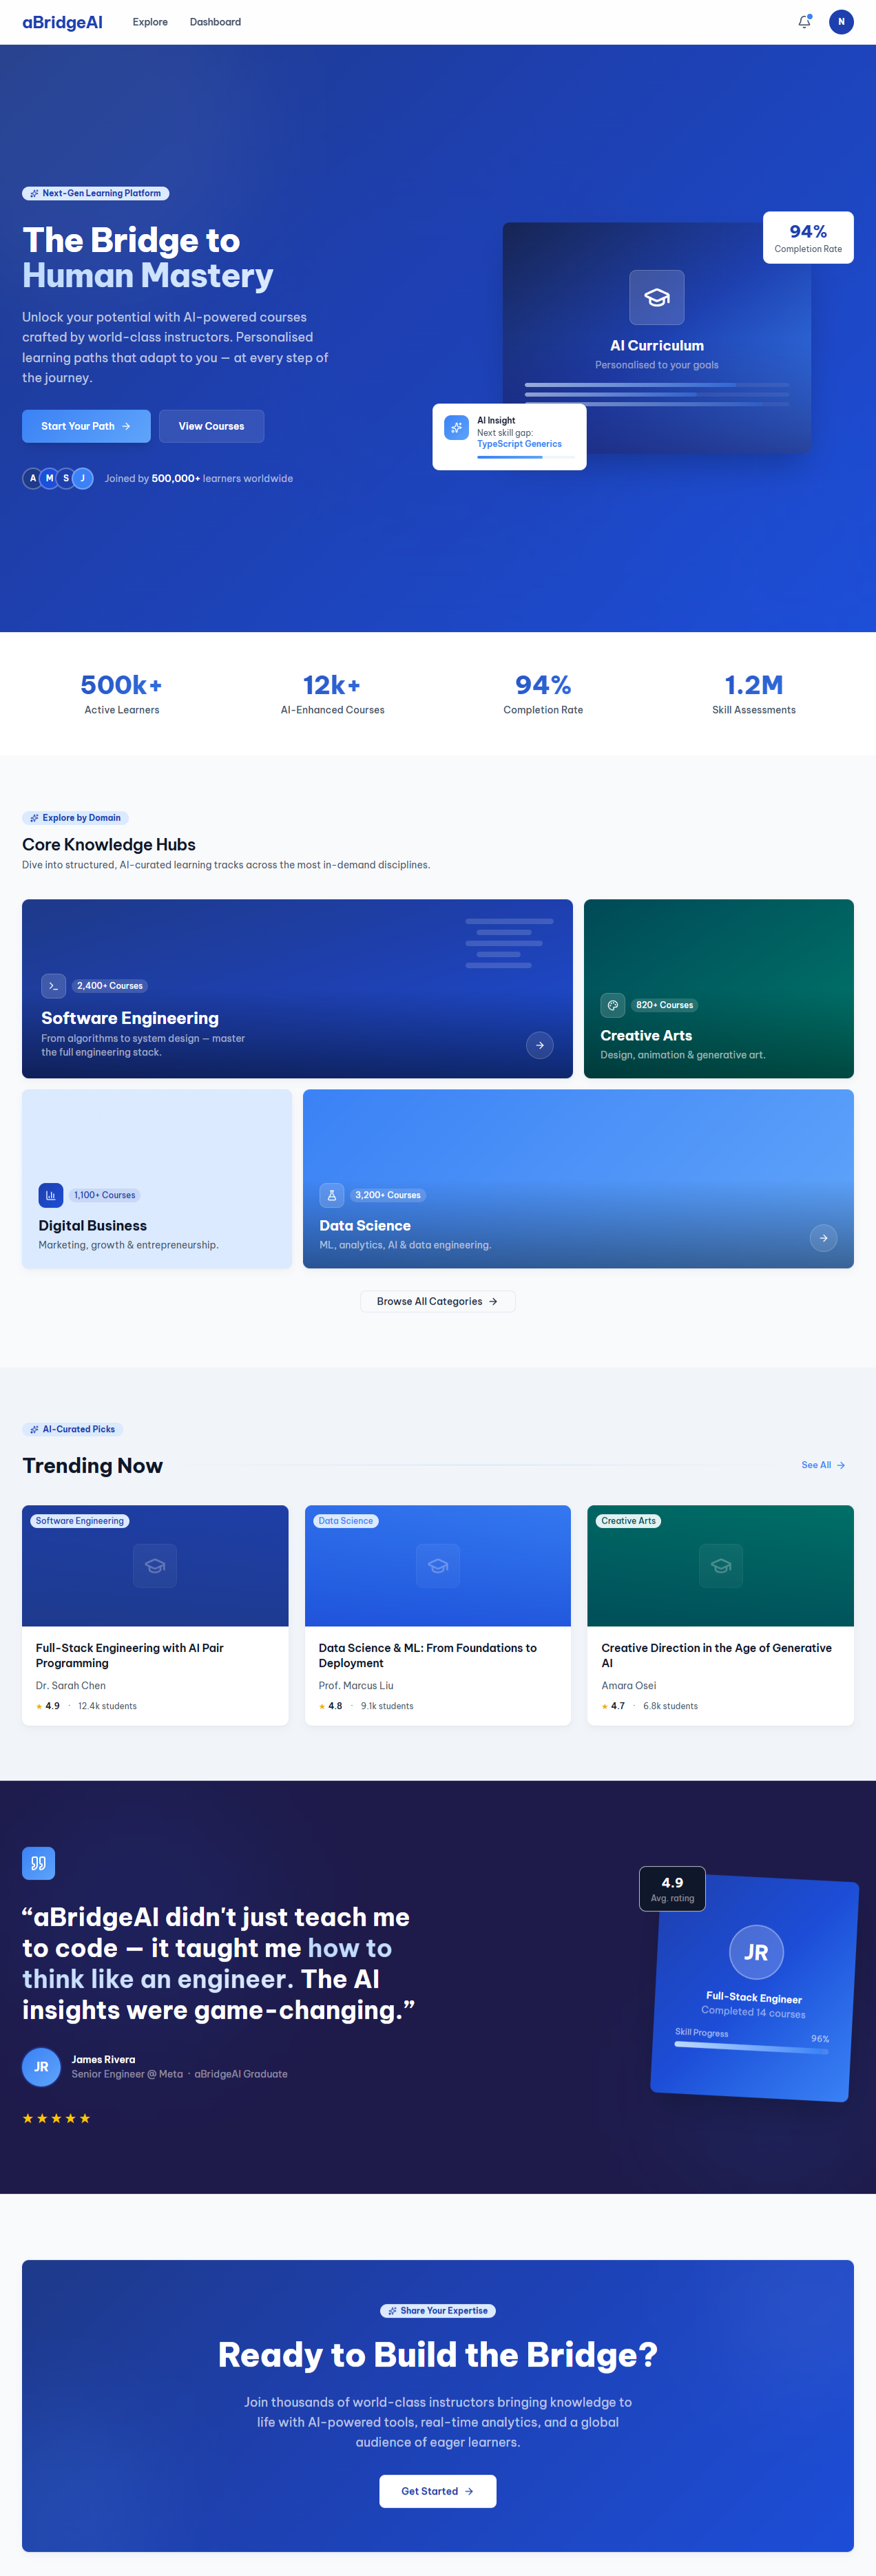
\includegraphics[width=\textwidth,height=0.85\textheight,keepaspectratio]{graphics/screenshots/01_landing_page.png}
  \caption{Landing Page --- Marketing entry point with hero section and call-to-action.}
  \label{fig:landing}
\end{figure}

The landing page is the public marketing surface. It carries a hero headline introducing the AI-powered career-readiness theme, a stats strip, a curated category grid, and a featured-courses carousel. Navigation links to the catalog, login, and sign-up flow are exposed in a horizontal \path|TopNavBar| that is unique to this page. The visual treatment is intentionally distinct from the authenticated shell so that crossing the login boundary feels like a deliberate handoff between marketing and product.

\paragraph{Authentication}

\begin{figure}[H]
  \centering
  \begin{minipage}{0.49\textwidth}
    
\includegraphics[width=\linewidth]{graphics/screenshots/02_login.png}
    \caption{Login --- Google SSO entry point.}
    \label{fig:login}
  \end{minipage}
\end{figure}

The login screen offers Google SSO as the single sign-in path; on successful redirect, the application checks whether the account has MFA configured and, if so, routes the user to \path|/login/mfa| for a TOTP or recovery-code challenge before issuing a session. A \path|next| query parameter preserves the originally requested route so deep links survive the auth round-trip.

% ── Student ─────────────────────────────────────────────────
\paragraph{Student Dashboard}

\begin{figure}[H]
  \centering
  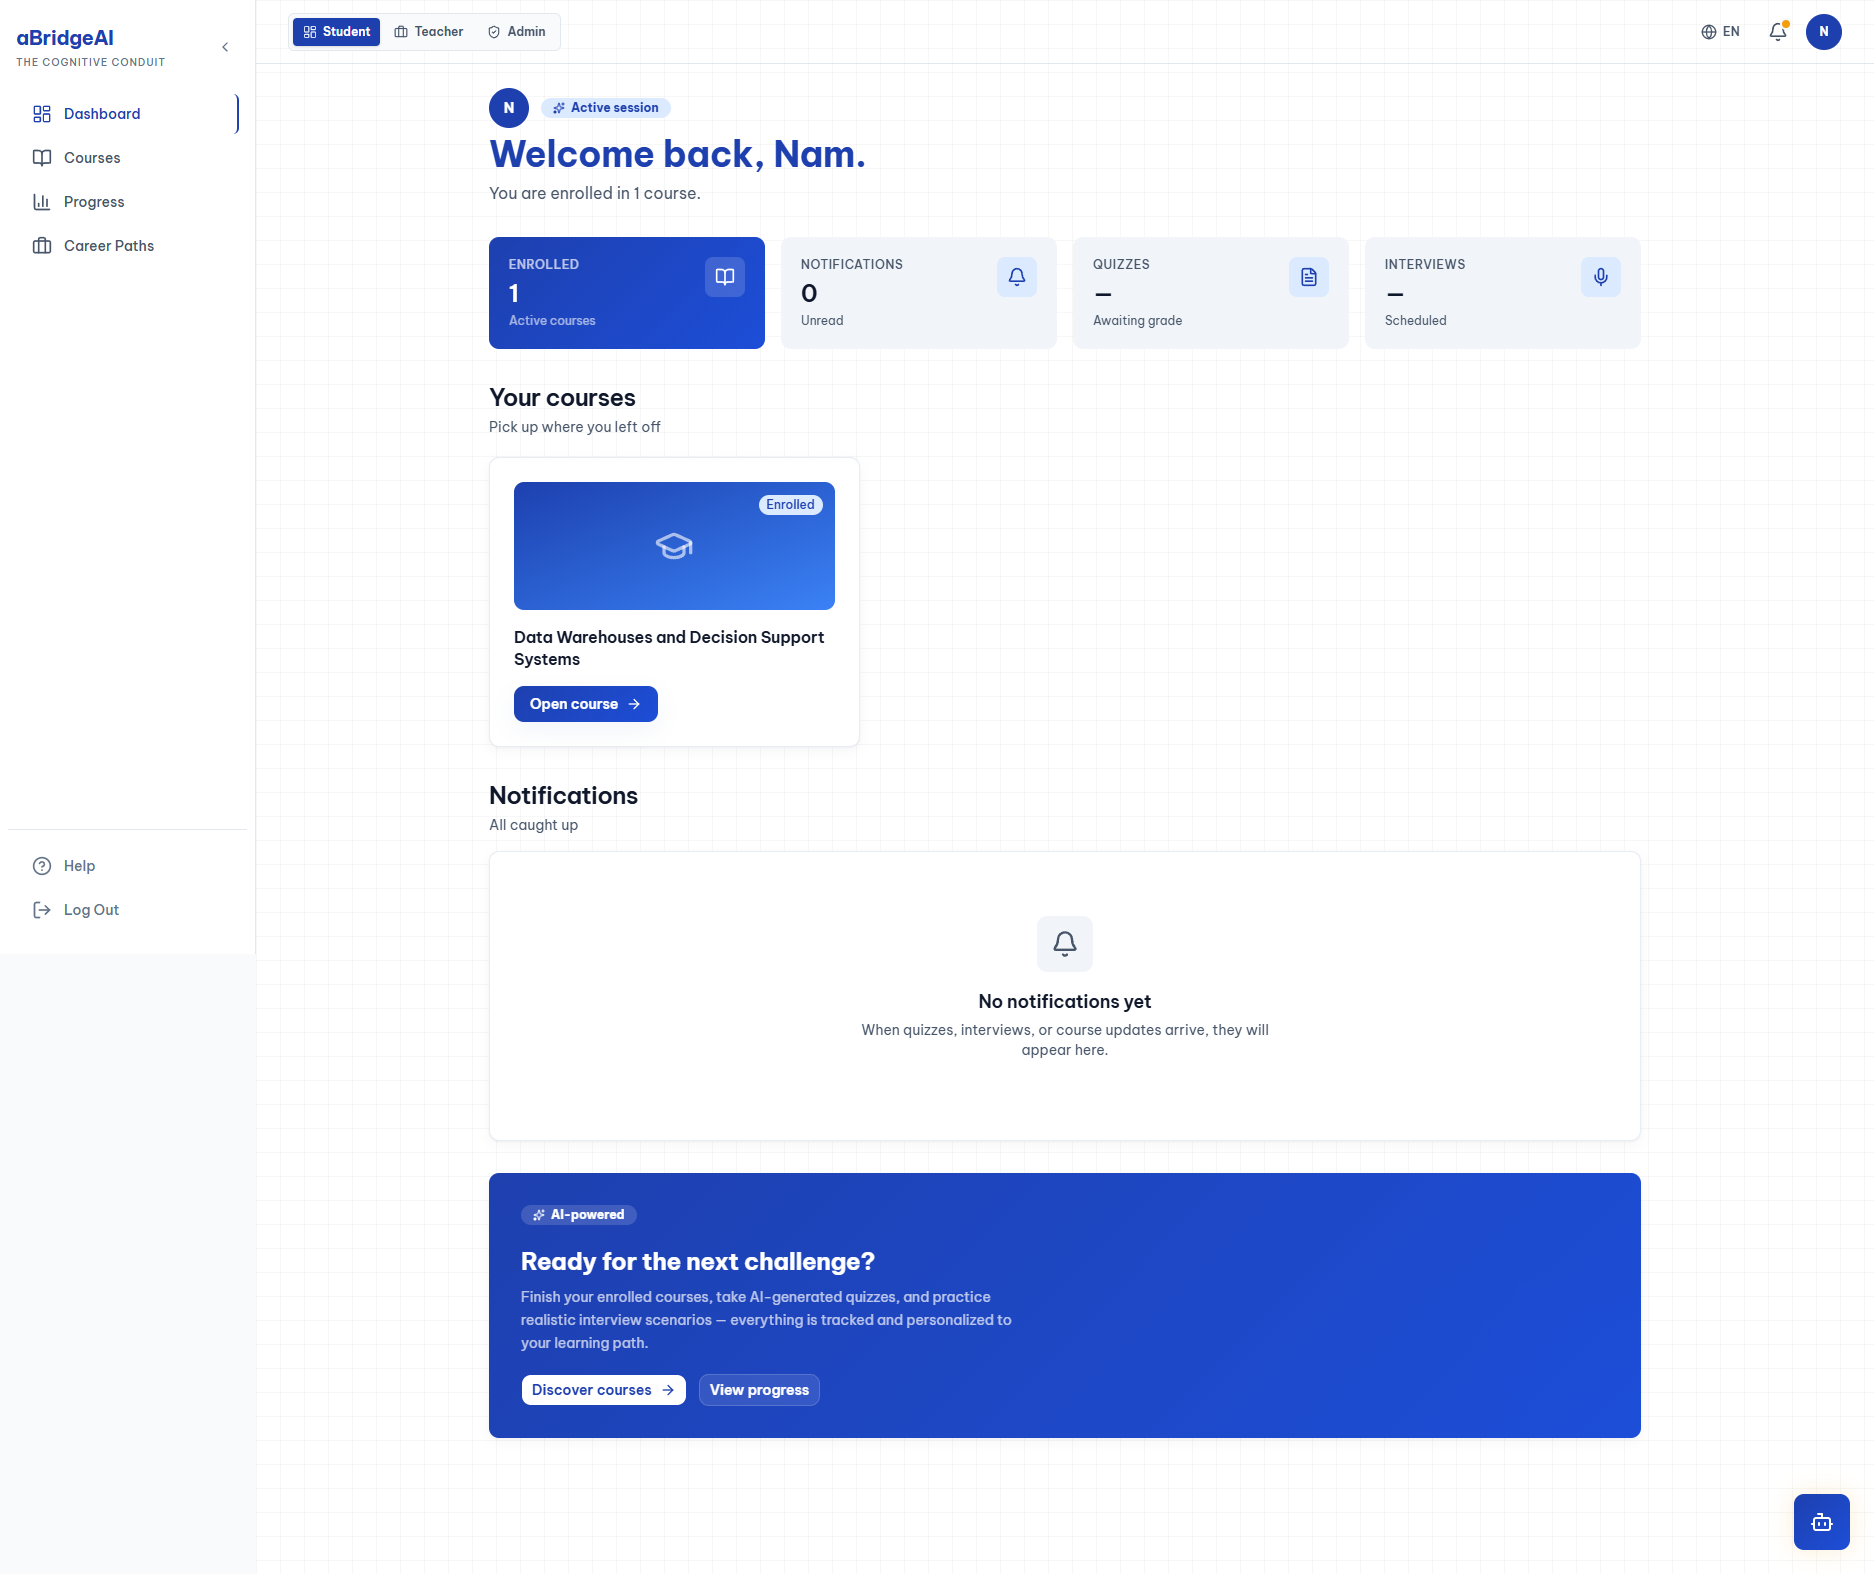
\includegraphics[width=\textwidth]{graphics/screenshots/04_student_dashboard.png}
  \caption{Student Dashboard --- Overview of enrolled courses, due reviews, and recent activity.}
  \label{fig:student_dashboard}
\end{figure}

The student dashboard surfaces only the information needed to decide what to study next. Stat cards summarise enrolled courses, in-progress lessons and recently earned badges; a recommendations strip suggests the next course in the active career path. The layout is intentionally calm --- there is no AI orb or floating action button --- to keep students focused on lesson work rather than ambient prompts.

\paragraph{Course Catalog}

\begin{figure}[H]
  \centering
  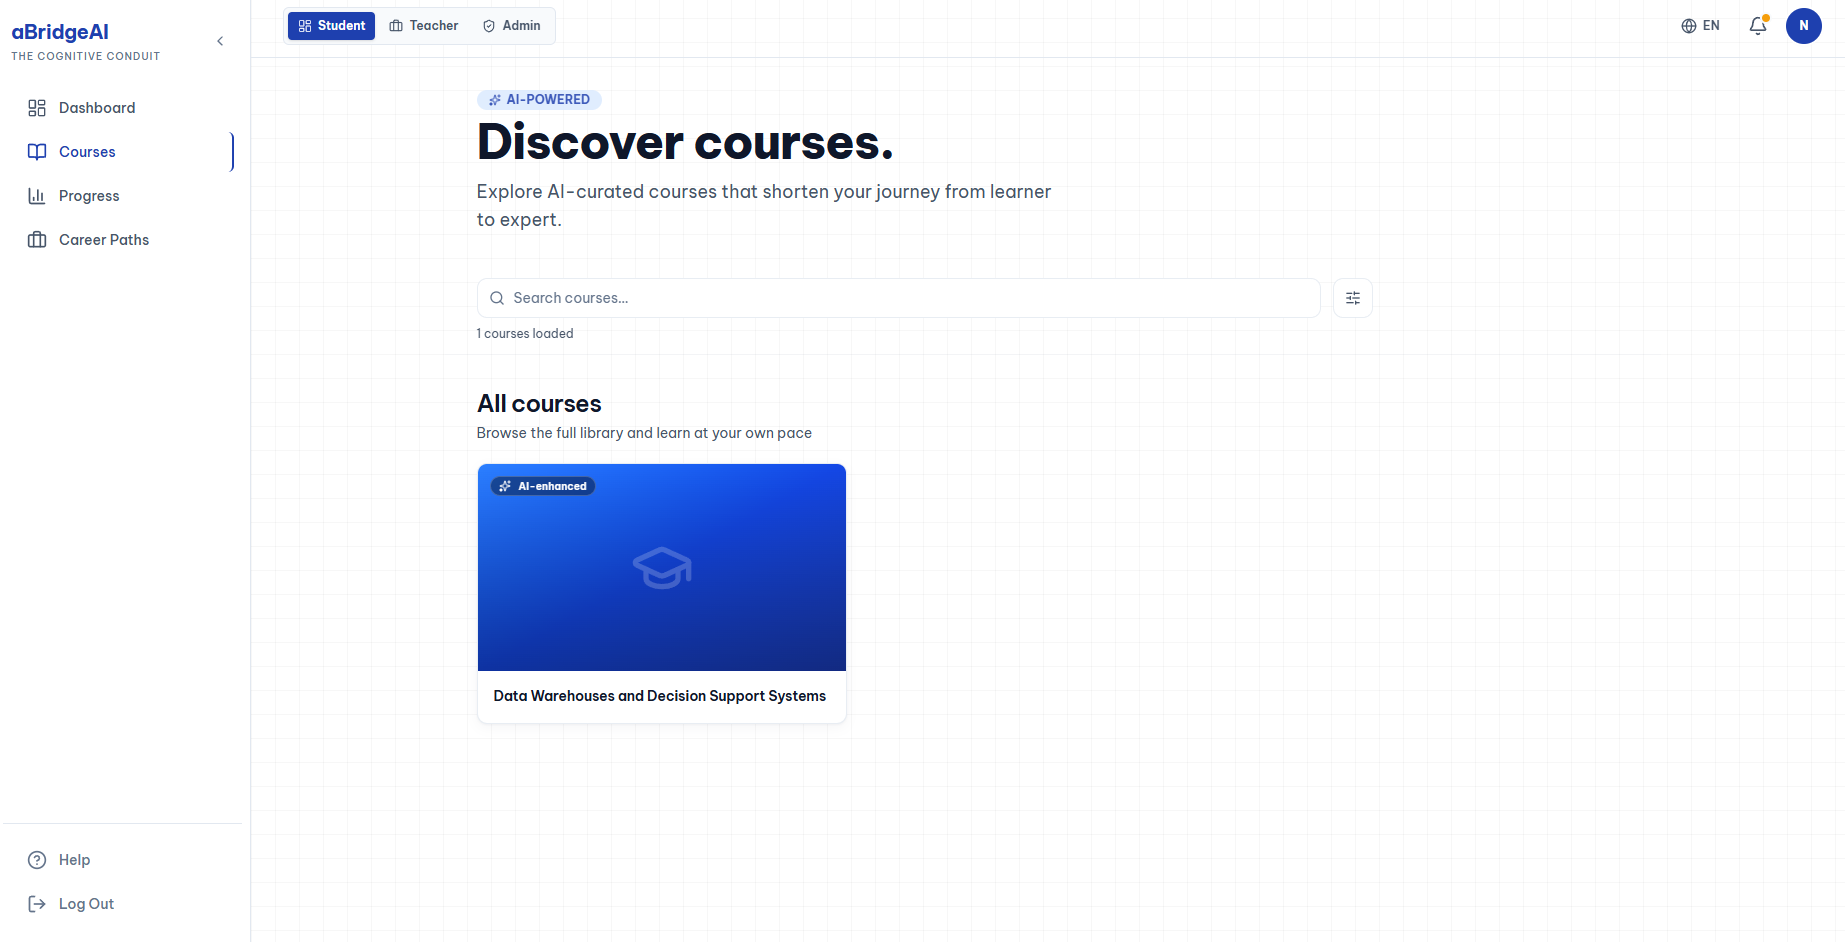
\includegraphics[width=\textwidth]{graphics/screenshots/05_course_catalog.png}
  \caption{Course Catalog --- Search, filter and enrollment status across the full course library.}
  \label{fig:course_catalog}
\end{figure}

The catalog opens with a sticky search and filter bar (query, category, difficulty), followed by a card grid that shows enrollment status and progress inline. Already-enrolled courses display a progress ring so students can pick up where they left off without leaving the catalog page.

\paragraph{Course View}

\begin{figure}[H]
  \centering
  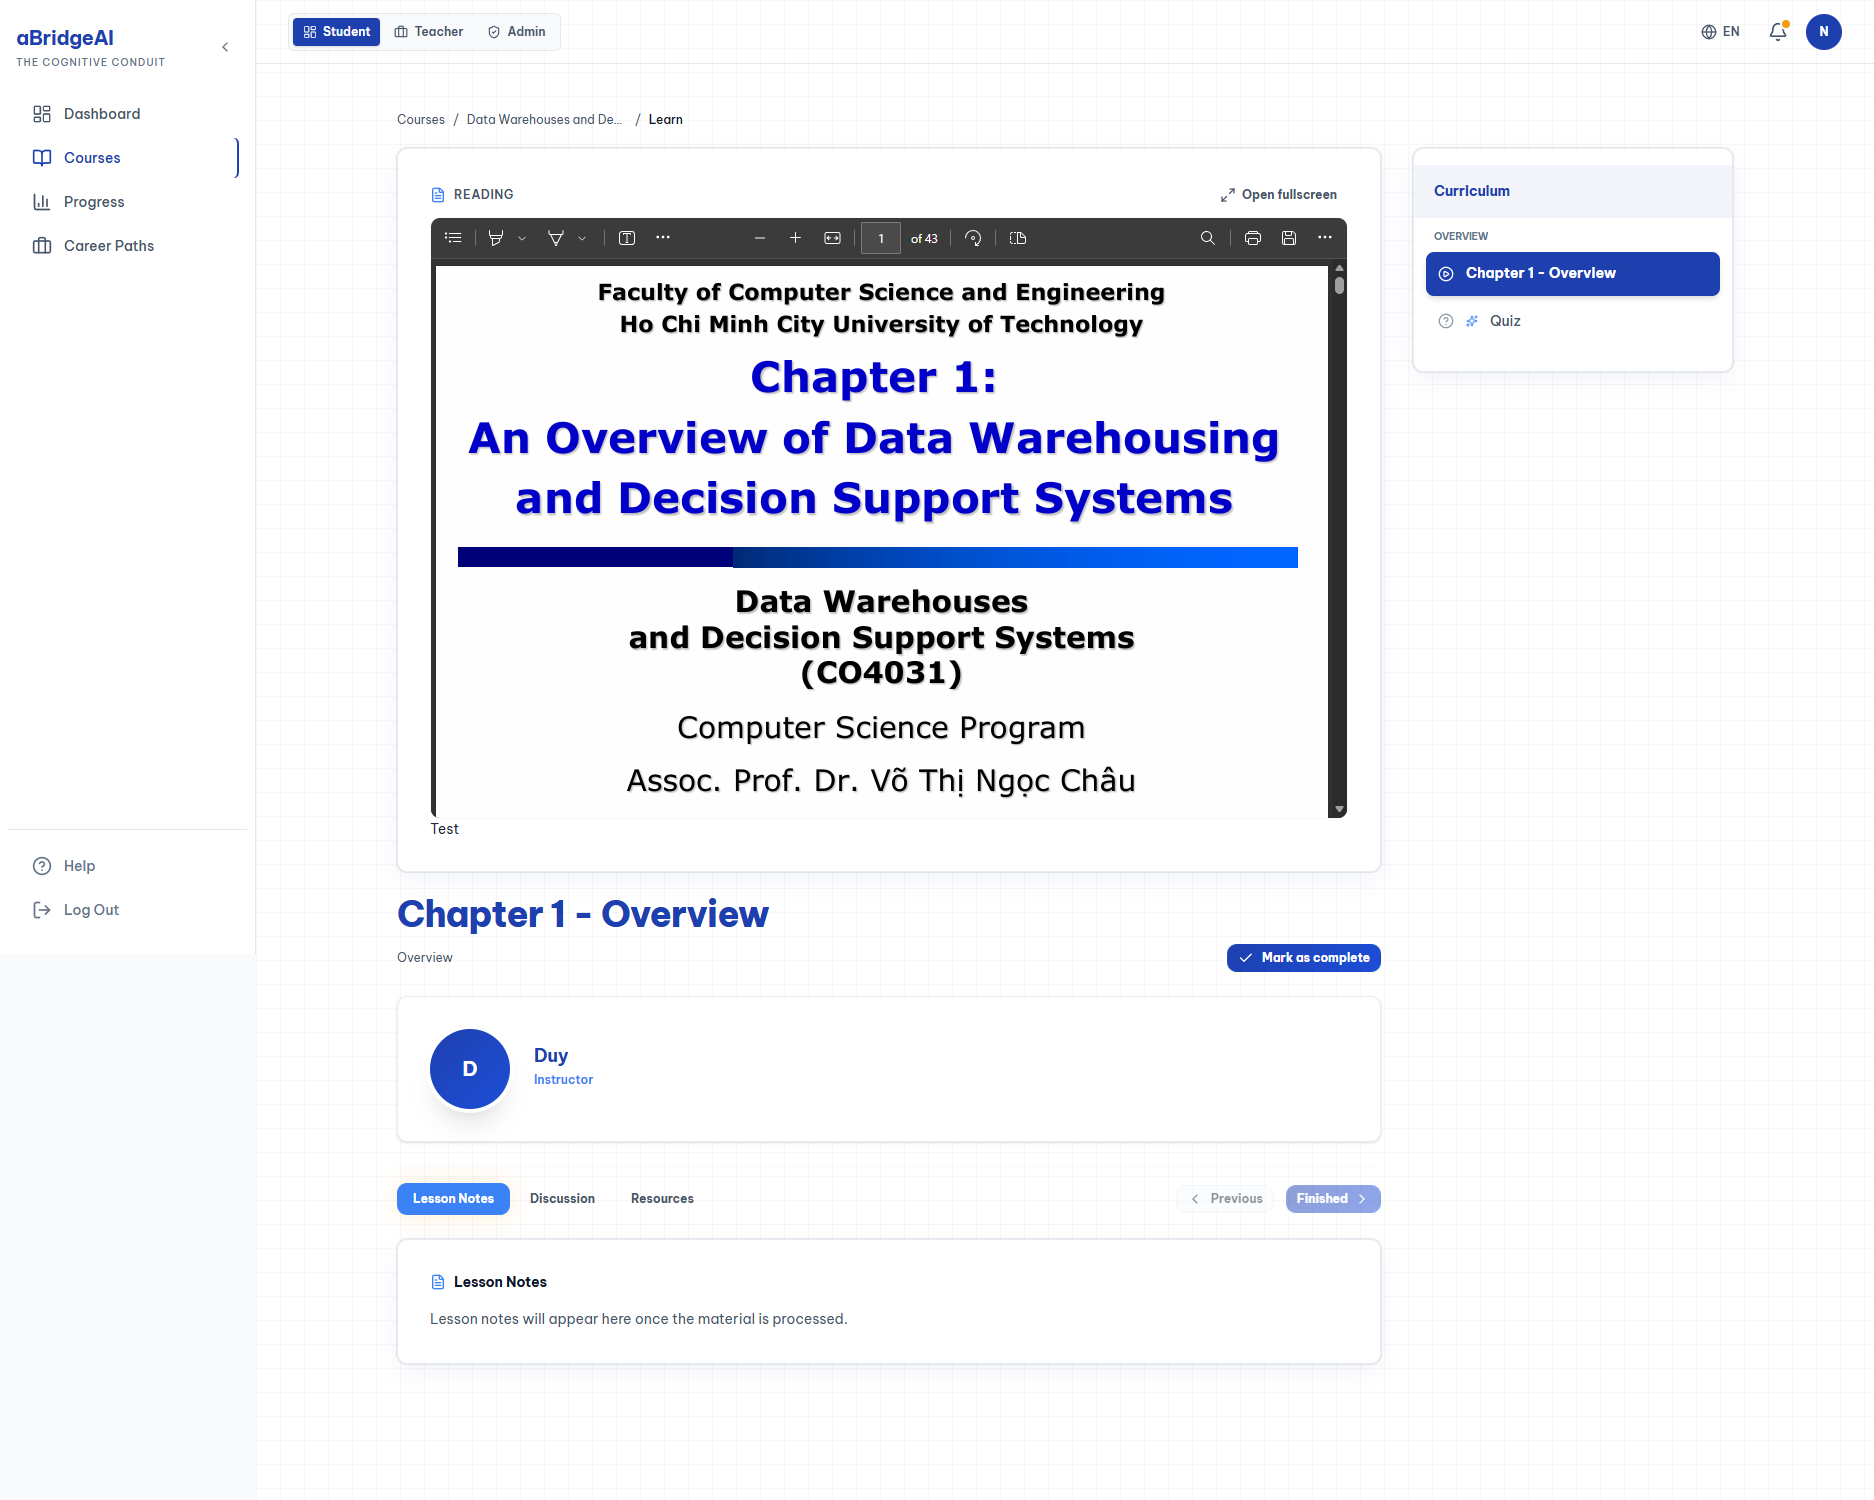
\includegraphics[width=\textwidth]{graphics/screenshots/06_course_view.png}
  \caption{Course View --- Curriculum accordion with lesson state icons.}
  \label{fig:course_view}
\end{figure}

The course view is the primary learning environment. The left panel hosts a sticky progress card and a curriculum accordion; each lesson displays its completion state (completed / active / locked / pending) via iconography. The right panel renders the active lesson's content --- video, reading, attached resources, or an embedded quiz launcher.

\paragraph{Quiz Session}

\begin{figure}[H]
  \centering
  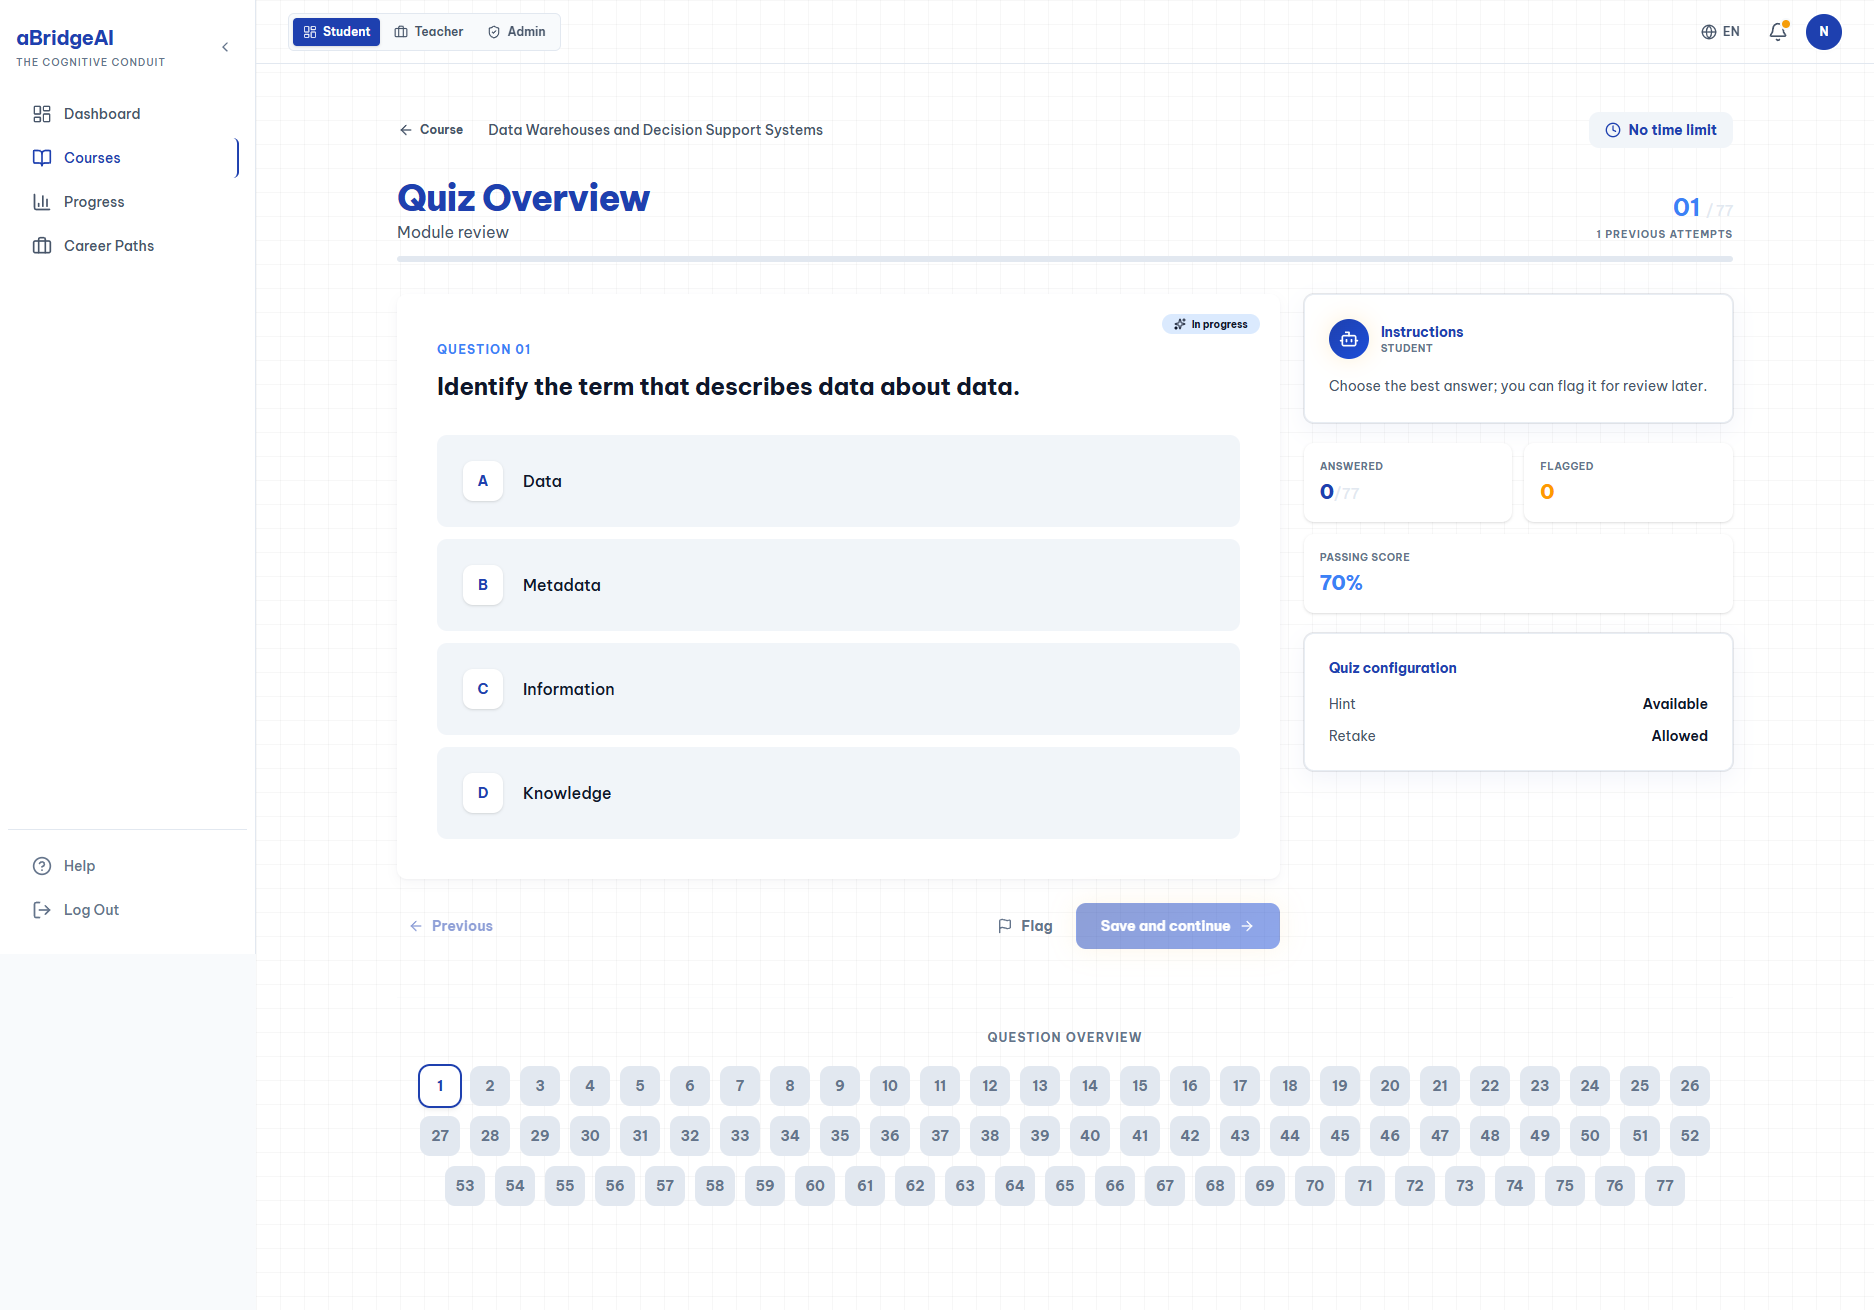
\includegraphics[width=\textwidth]{graphics/screenshots/07_student_quiz.png}
  \caption{Quiz Session --- Timed multiple-choice interface with question navigation.}
  \label{fig:student_quiz}
\end{figure}

The quiz session is a focused, distraction-free interface. A countdown timer at the top creates temporal urgency; the bottom question grid allows non-linear navigation between flagged or unanswered items. After submission, students are redirected to the attempt-review screen at \path|/courses/$slug/quiz/$quizId/attempts/$attemptId|, which renders correct answers and per-question explanations.

% ── Instructor ──────────────────────────────────────────────
\paragraph{Teacher Dashboard}

\begin{figure}[H]
  \centering
  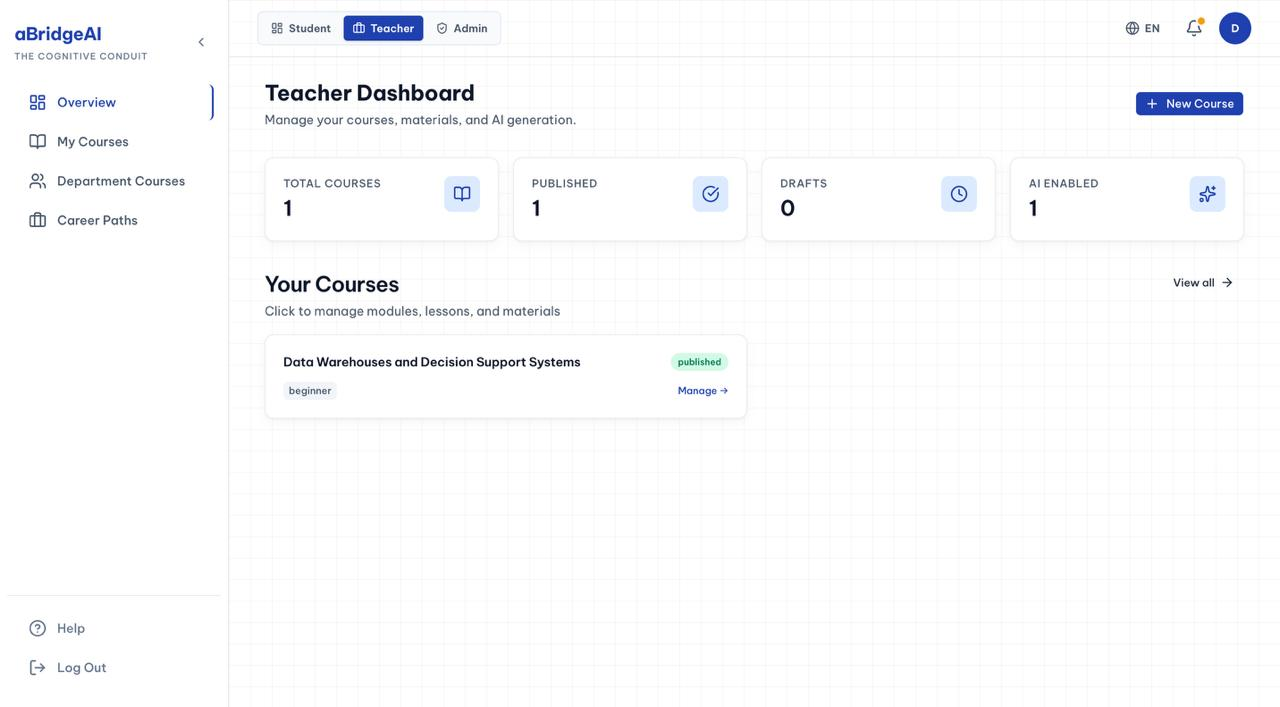
\includegraphics[width=\textwidth]{graphics/screenshots/14_instructor_dashboard.png}
  \caption{Teacher Dashboard --- Operational overview with course health stats and quick course creation.}
  \label{fig:instructor_dashboard}
\end{figure}

The teacher dashboard is the entry screen for the \path|/teacher| route group. Four stat cards summarise the instructor's authoring activity --- total courses, published, drafts, and AI-enabled --- followed by a ``Your Courses'' strip that surfaces the most recently edited course with its difficulty tag and publish state. A primary \textbf{+ New Course} button anchors the top-right corner, and a \textbf{Manage} link on each course card jumps directly into the course-management view. The role switcher (Student / Teacher / Admin) at the top of the page is a development affordance for users that hold multiple roles; production accounts only see the tabs they are entitled to.

\paragraph{Course Management}

\begin{figure}[H]
  \centering
  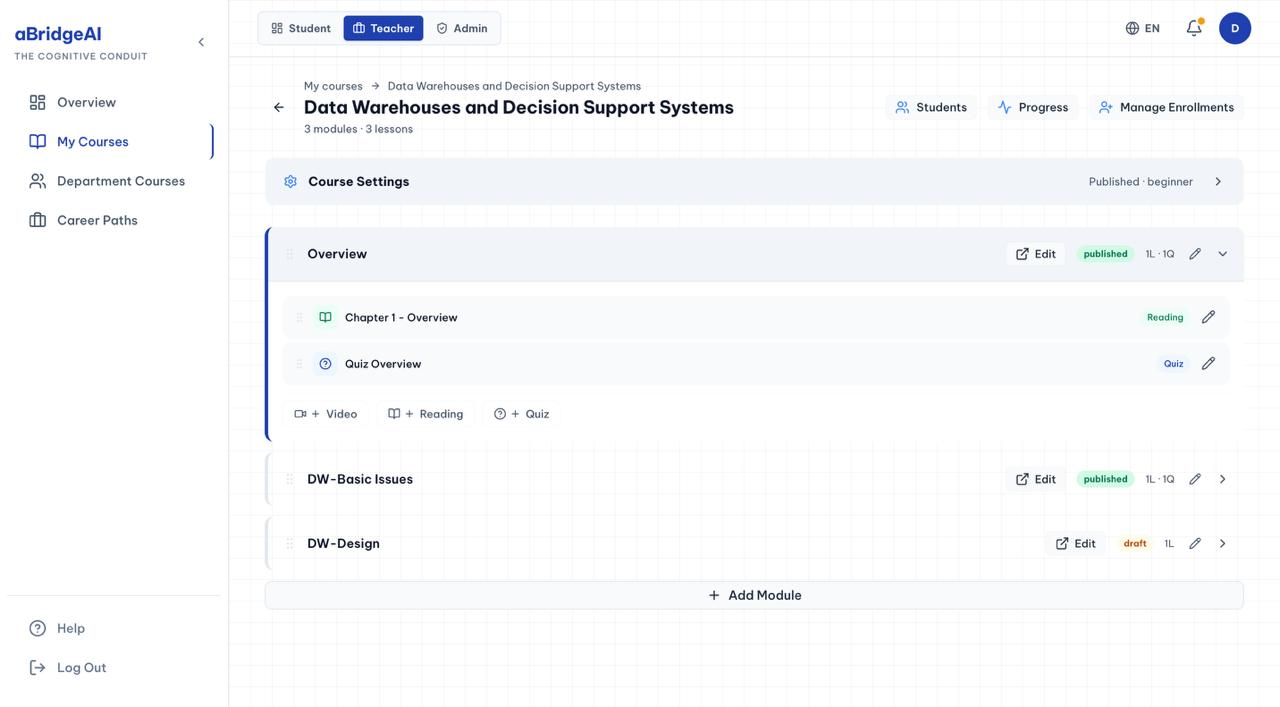
\includegraphics[width=\textwidth]{graphics/screenshots/instructor_course_manage.png}
  \caption{Course Manage --- Module and lesson tree with drag-handle reordering and inline quick-add.}
  \label{fig:instructor_course_manage}
\end{figure}

The course-management page (\path|/teacher/courses/$courseId|) is the authoring core of the platform. Modules render as collapsible cards in a drag-handle list; expanding a module reveals its ordered lesson and quiz items, each carrying a publish-state badge. Inline \textbf{+ Video}, \textbf{+ Reading} and \textbf{+ Quiz} buttons let the instructor grow the curriculum without leaving the page. A right-hand \textit{Course Settings} panel exposes the publish toggle, difficulty, and Students / Progress / Manage Enrollments quick links. A bottom \textbf{+ Add Module} button extends the structure.

\paragraph{Lesson Editor}

\begin{figure}[H]
  \centering
  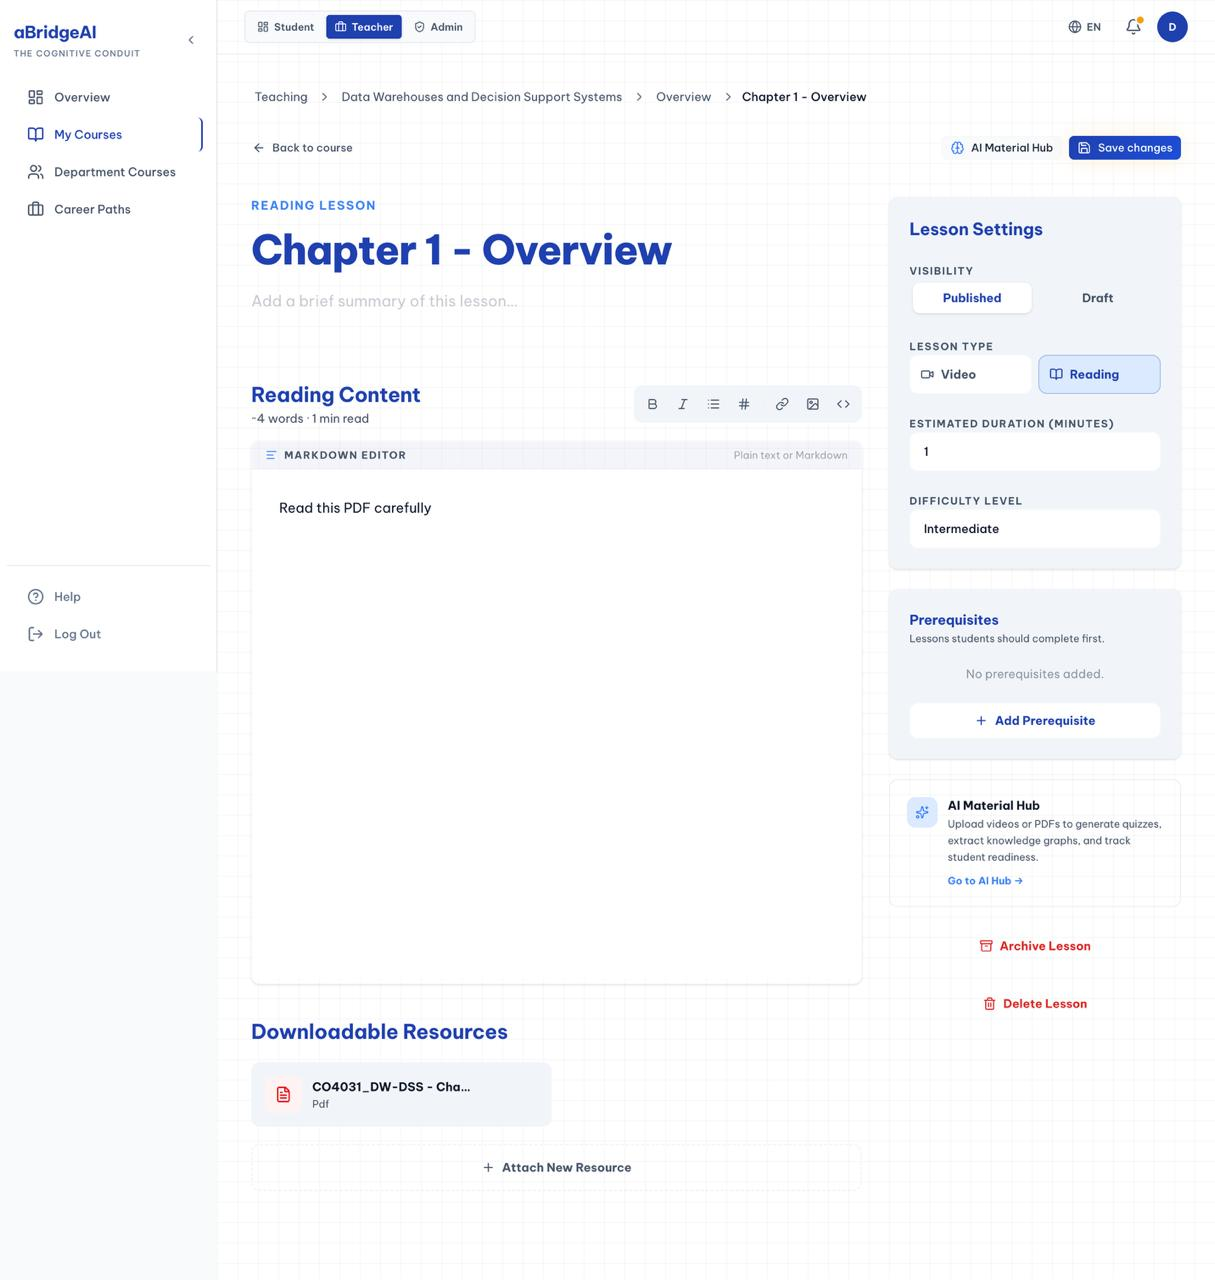
\includegraphics[width=\textwidth]{graphics/screenshots/instructor_lesson_manage.png}
  \caption{Lesson Editor --- Markdown content editor with attached resources and right-hand settings panel.}
  \label{fig:instructor_lesson_manage}
\end{figure}

The lesson editor (\path|/teacher/courses/$courseId/lessons/$lessonId|) is split into a content area and a settings sidebar. The left side shows a Markdown editor for reading lessons (with bold, italic, list, heading, link, image, and code controls) and a \textit{Downloadable Resources} block for attached PDFs and other files. The right sidebar exposes Visibility (Published / Draft), Lesson Type (Video / Reading), Estimated Duration, Difficulty Level, and a Prerequisites picker. An \textit{AI Material Hub} card promotes uploading source material so the platform can auto-generate quizzes from it. Destructive actions (Archive, Delete) are pushed to the bottom of the sidebar to reduce mis-clicks. A persistent \textbf{Save changes} button anchors the top-right corner.

\paragraph{Quiz Editor}

\begin{figure}[H]
  \centering
  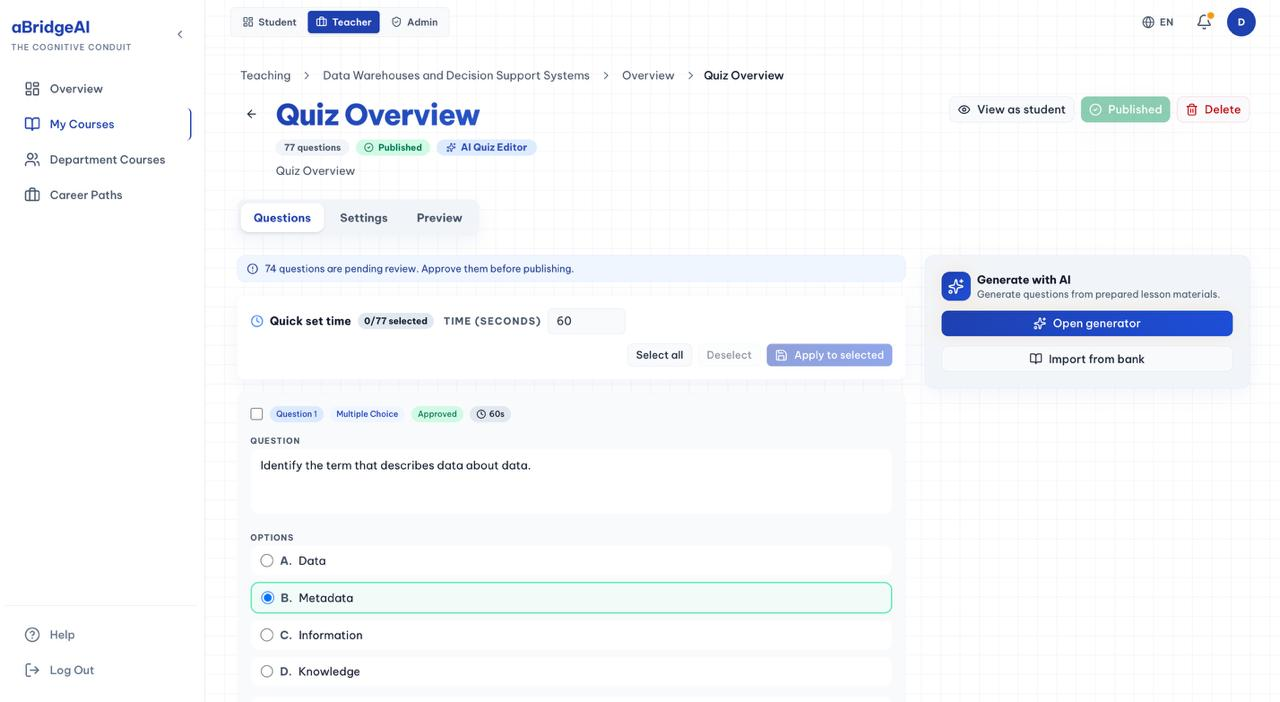
\includegraphics[width=\textwidth]{graphics/screenshots/24_quiz_editor.png}
  \caption{Quiz Editor --- Question list with bulk timing controls and an AI-generation side panel.}
  \label{fig:instructor_quiz_editor}
\end{figure}

The quiz editor (\path|/teacher/courses/$courseId/quizzes/$quizId|) is structured around three sub-tabs: \textbf{Questions} (active by default), \textbf{Settings}, and \textbf{Preview}. The Questions tab lists every item with its type badge (Multiple Choice, True/False, \dots), per-question time limit, and approval status. A bulk-action toolbar lets instructors select multiple questions and apply a uniform time limit, approve in bulk, or delete. A persistent banner reports how many questions are pending review (e.g.\ ``74 questions are pending review --- approve them before publishing''), enforcing a deliberate approval gate between AI generation and student exposure.

\paragraph{AI Quiz Generation}

\begin{figure}[H]
  \centering
  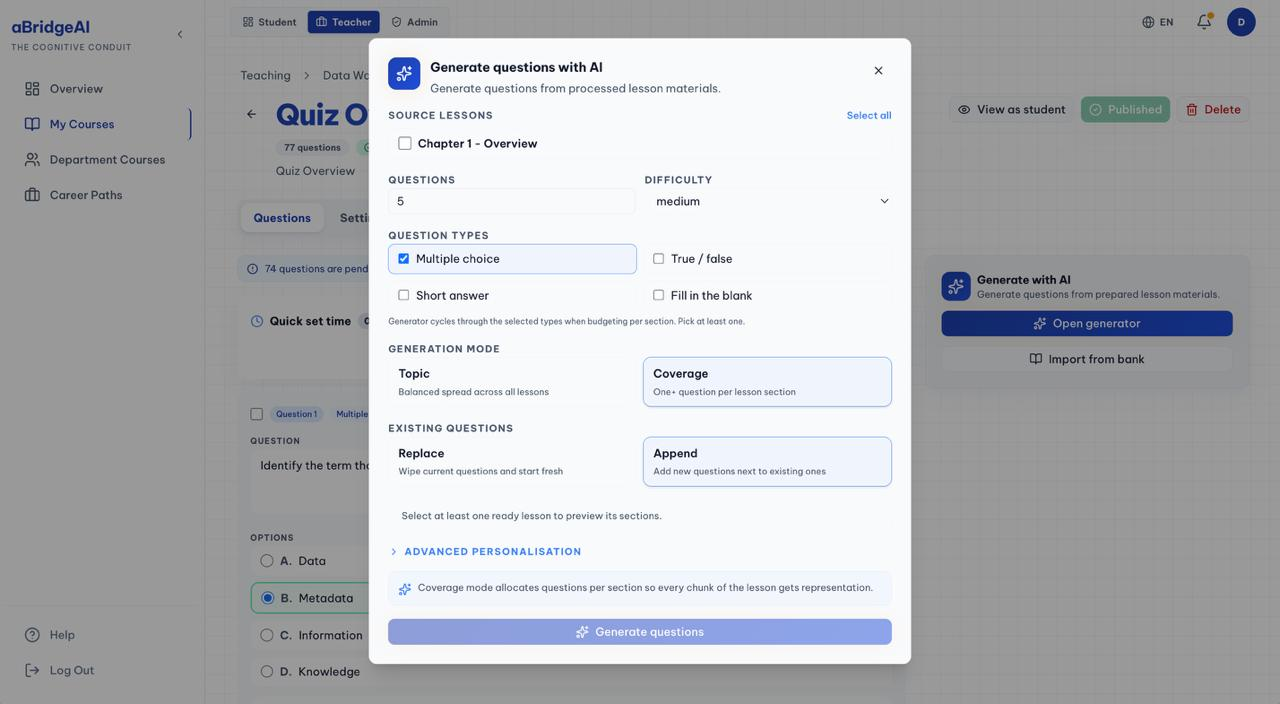
\includegraphics[width=0.85\textwidth]{graphics/screenshots/instructor_quiz_ai_modal.png}
  \caption{AI Quiz Generation modal --- Source-lesson selection, question count, mode and append/replace controls.}
  \label{fig:instructor_quiz_ai}
\end{figure}

The \textbf{Open generator} button on the quiz editor opens a modal that drives the AI quiz pipeline. The instructor selects one or more source lessons (only lessons whose materials have been processed are eligible), the desired number of questions, the difficulty band, and the question types (Multiple choice, True/False, Short answer, Fill in the blank). A generation-mode selector trades off two strategies: \textit{Topic} produces a balanced spread across all selected lessons, while \textit{Coverage} guarantees at least one question per section. An existing-questions selector decides between \textit{Replace} (wipe and regenerate) and \textit{Append} (add to the current bank). An advanced personalisation block, collapsed by default, exposes per-attempt prompt controls. Generated questions land in the editor in a \textit{Pending Review} state and only become visible to students after explicit instructor approval.

% ── Administrator ───────────────────────────────────────────
\paragraph{Processing Queue}

\begin{figure}[H]
  \centering
  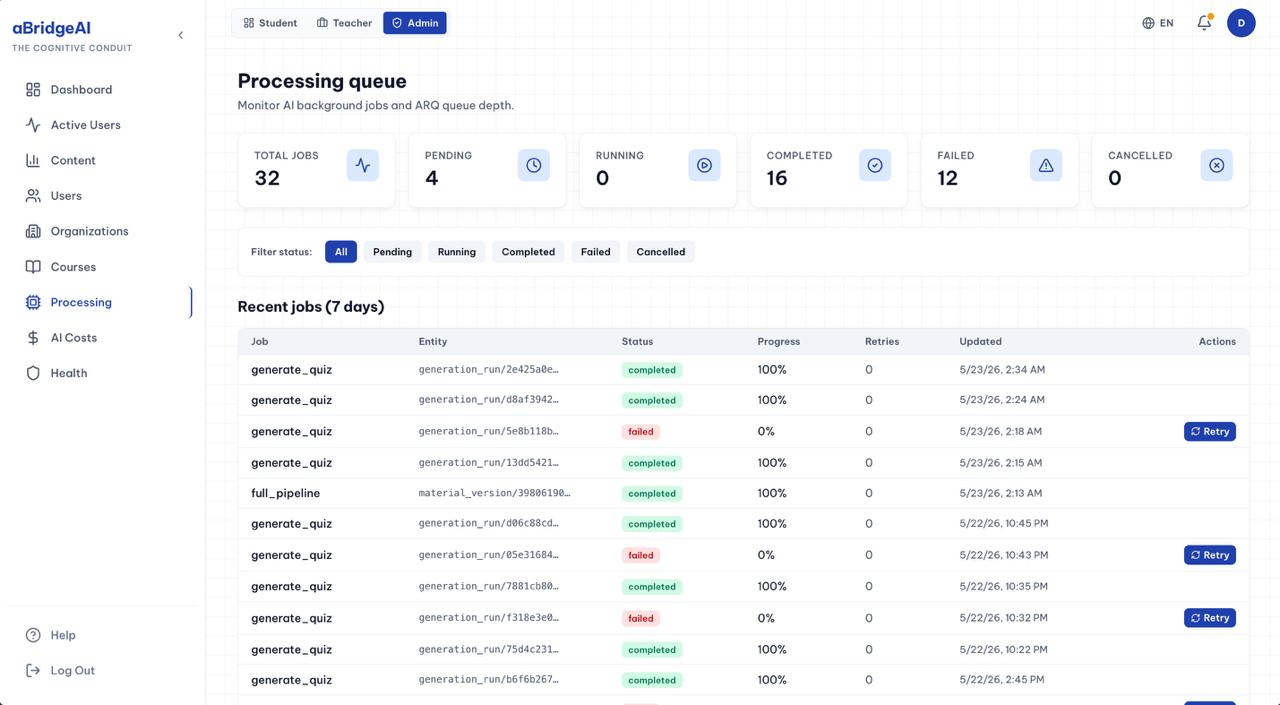
\includegraphics[width=\textwidth]{graphics/screenshots/admin_processing.png}
  \caption{Admin Processing Queue --- Background-job visibility with retry actions for failed runs.}
  \label{fig:admin_processing}
\end{figure}

The processing queue (\path|/admin/processing|) gives platform administrators direct visibility into the AI background-job pipeline (material ingestion, embedding, quiz generation, validation). Stat cards report the current backlog (Total, Pending, Running, Completed, Failed, Cancelled). A status-pill filter (\textit{All}, \textit{Pending}, \textit{Running}, \textit{Completed}, \textit{Failed}, \textit{Cancelled}) narrows the table, which lists the job type (\path|generate_quiz|, \path|full_pipeline|, \dots), the target entity ID, status, progress, retry count, last update, and a per-row \textbf{Retry} action for failed jobs. This is the operations console for the worker tier; it complements the per-course \textit{AI Material Hub} indicator visible to instructors.

\paragraph{AI Costs}

\begin{figure}[H]
  \centering
  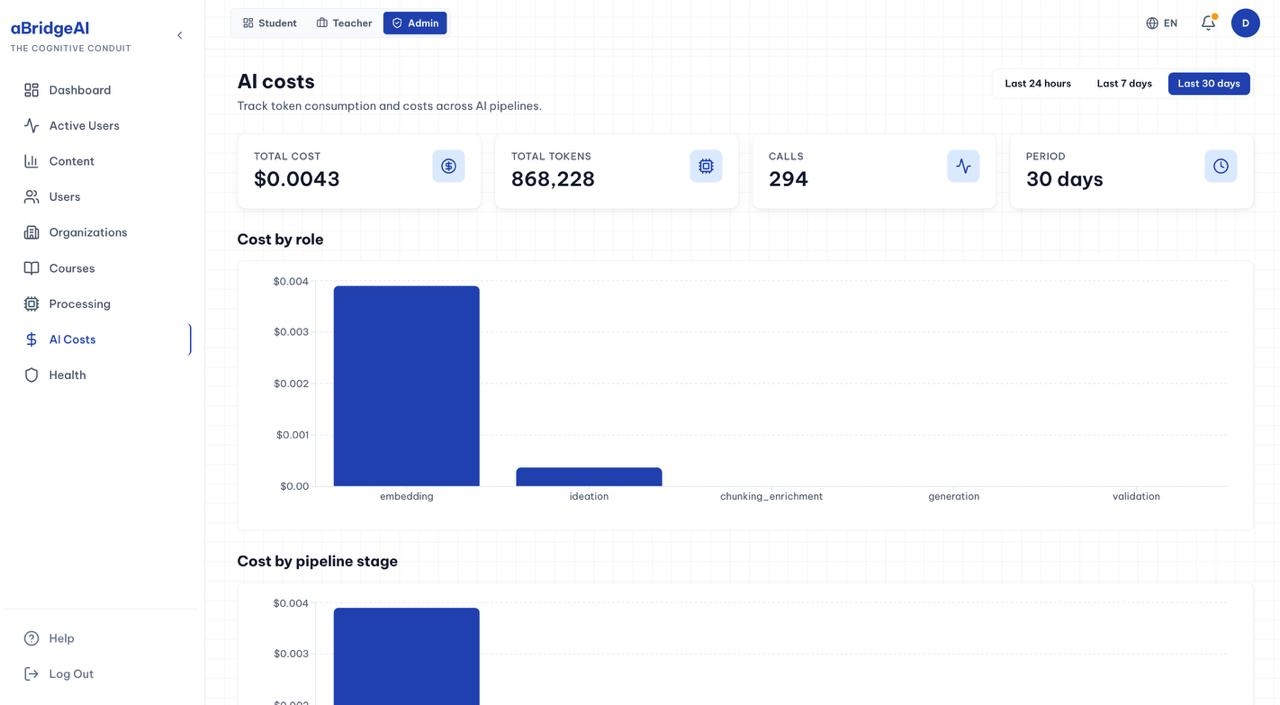
\includegraphics[width=\textwidth]{graphics/screenshots/admin_ai_costs.png}
  \caption{Admin AI Costs --- Token consumption and spend across pipeline roles and stages.}
  \label{fig:admin_ai_costs}
\end{figure}

The AI Costs page (\path|/admin/ai-costs|) exposes platform-wide spend on language-model and embedding APIs. A time-range selector (Last 24 hours, Last 7 days, Last 30 days) refilters every metric on the page. Summary cards report Total Cost, Total Tokens, total API Calls, and the active period. Two bar charts break the spend down by \textit{role} (embedding, ideation, chunking enrichment, generation, validation) and by \textit{pipeline stage}. The chart series reuse the platform palette (academic blue + amber) so administrators can correlate cost with backlog health on the Processing page without a context switch.

% ────────────────────────────────────────────────────────────
\subsubsection{Navigation Architecture}
% ────────────────────────────────────────────────────────────

\begin{longtable}{|p{0.22\textwidth}|p{0.20\textwidth}|p{0.46\textwidth}|}
  \caption{Navigation Components by Context} \label{tab:nav_components} \\
  \hline
  \textbf{Component} & \textbf{Context} & \textbf{Function} \\
  \hline
  \endfirsthead
  \multicolumn{3}{c}{\small\tablename~\thetable{} \textit{(continued)}} \\
  \hline
  \textbf{Component} & \textbf{Context} & \textbf{Function} \\
  \hline
  \endhead
  \hline
  \endfoot
  \path|TopNavBar| & Landing page only & Horizontal marketing nav: Explore, Login, Sign Up. Distinct from the authenticated shell. \\
  \hline
  \path|SideNavBar| & Authenticated (all) & Always rendered. Collapses to \path|w-16| (icons only) below the \path|md| breakpoint or by user toggle; expands to \path|w-64| with full labels. Receives a role-specific \path|navItems| array as a prop. \\
  \hline
  \path|ContentTopBar| & Authenticated (all) & Sticky page header carrying the current page title, language selector (i18n), notification bell, and user avatar with menu. \\
  \hline
  \path|AppShell| & Authenticated (all) & Orchestrates \path|SideNavBar| + \path|ContentTopBar| + main content into a responsive layout. Receives a \path|navItems| array, making it fully reusable across student, teacher, and admin route groups with no per-role layout code. \\
  \hline
  \path|Footer| & Landing page only & Marketing footer with product links and legal copy. \\
  \hline
\end{longtable}

The \path|AppShell| component is the structural keystone of the authenticated experience. The shell itself is role-agnostic; role differentiation is communicated through the \path|navItems| prop (defined in \path|src/lib/navigation.ts|) and through the active accent colour on the sidebar. Below the \path|md| breakpoint the sidebar overlays the page content via a backdrop rather than pushing it, keeping the main column readable on narrow screens.

% ────────────────────────────────────────────────────────────
\subsubsection{Design System Summary}
% ────────────────────────────────────────────────────────────

\begin{longtable}{|p{0.22\textwidth}|p{0.30\textwidth}|p{0.36\textwidth}|}
  \caption{Design System Tokens} \label{tab:design_tokens} \\
  \hline
  \textbf{Token Category} & \textbf{Value} & \textbf{Usage} \\
  \hline
  \endfirsthead
  \multicolumn{3}{c}{\small\tablename~\thetable{} \textit{(continued)}} \\
  \hline
  \textbf{Token Category} & \textbf{Value} & \textbf{Usage} \\
  \hline
  \endhead
  \hline
  \endfoot
  Page background & \path|#f8fafc| (slate-50) & Page surface in light mode. \\
  \hline
  Surface / Card & \path|#ffffff| & Cards, panels, dialogs. \\
  \hline
  Primary accent & \path|#1e40af| (blue-800) & Primary actions, active nav, links, chart series 1. \\
  \hline
  Secondary accent & \path|#3b82f6| (blue-500) & Secondary buttons, focus rings, chart series 2. \\
  \hline
  CTA / accent & \path|#f59e0b| (amber-500) & High-attention CTAs, AI affordances. \\
  \hline
  Success & \path|#16a34a| (green-600) & Published / completed state. \\
  \hline
  Warning & \path|#ea580c| (orange-600) & Drafts, pending review. \\
  \hline
  Danger & \path|#dc2626| (red-600) & Failed jobs, destructive actions. \\
  \hline
  Border & \path|#e2e8f0| (slate-200) & 1\,px borders on cards, inputs, tables. \\
  \hline
  Typography & Be Vietnam Pro (system-ui fallback) & All body and UI text; full Vietnamese diacritic support. \\
  \hline
  Component library & shadcn/ui + Radix UI & Dialogs, dropdowns, sheets, tooltips. \\
  \hline
  Icons & Lucide React & Single iconography source across the platform. \\
  \hline
  Charts & Recharts & Bar, line, area; reuses palette for chart series 1--5. \\
  \hline
  i18n keys & \path|src/lib/navigation.ts| + \path|src/locales/<lang>.json| & Translatable nav labels and copy. \\
  \hline
  Max modal depth & 1 stacked modal & Prevents nested-modal anti-patterns. \\
  \hline
  Base spacing unit & 4\,px & All spacing is a multiple of 4\,px. \\
  \hline
  Border radius (card) & 8\,px (\path|rounded-lg|) & Consistent card rounding; 10\,px hard cap project-wide. \\
  \hline
  Sidebar widths & 64\,px collapsed / 256\,px expanded & \path|w-16| / \path|w-64|; collapse driven by viewport width and user toggle. \\
  \hline
\end{longtable}
